\documentclass[tikz,border=2pt]{standalone}
\usepackage{amsmath}
\usetikzlibrary{arrows.meta}
\begin{document}
% Correlated common prior p on {a,b} x {x,y}: player 1's beliefs condition on a row
% (p(x|a)=0.4/0.5=0.8, p(x|b)=0.2/0.5=0.4), player 2's on a column (p(a|x)=0.4/0.6=2/3, p(a|y)=0.1/0.4=1/4).
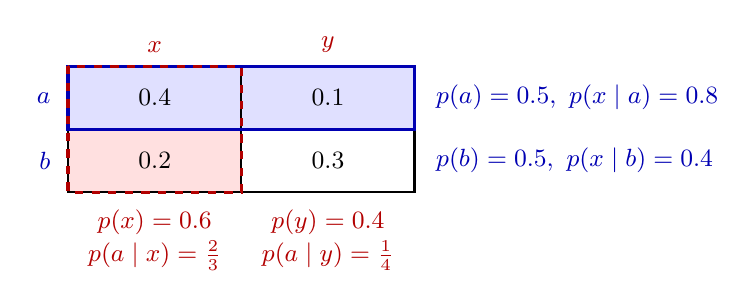
\begin{tikzpicture}[font=\small, >={Latex[length=2mm]}]
  \def\w{2.2} \def\h{0.8}
  % row a (player 1, type a) and column x (player 2, type x)
  \fill[blue!12] (0,0) rectangle (2*\w,-\h);
  \fill[red!12] (0,0) rectangle (\w,-2*\h);
  \fill[blue!12] (0,0) rectangle (\w,-\h);
  \draw[thick] (0,0) rectangle (2*\w,-2*\h);
  \draw[thick] (\w,0) -- (\w,-2*\h);
  \draw[thick] (0,-\h) -- (2*\w,-\h);
  \draw[blue!70!black, very thick] (0,0) rectangle (2*\w,-\h);
  \draw[red!70!black, very thick, dashed] (0,0) rectangle (\w,-2*\h);
  % headers
  \node[red!70!black, anchor=south] at (0.5*\w,0.05) {$x$};
  \node[red!70!black, anchor=south] at (1.5*\w,0.05) {$y$};
  \node[blue!70!black, anchor=east] at (-0.1,-0.5*\h) {$a$};
  \node[blue!70!black, anchor=east] at (-0.1,-1.5*\h) {$b$};
  % joint probabilities
  \node at (0.5*\w,-0.5*\h) {$0.4$};
  \node at (1.5*\w,-0.5*\h) {$0.1$};
  \node at (0.5*\w,-1.5*\h) {$0.2$};
  \node at (1.5*\w,-1.5*\h) {$0.3$};
  % player 1: condition on the row
  \node[blue!70!black, anchor=west] at (2*\w+0.15,-0.5*\h) {$p(a)=0.5,\ p(x\mid a)=0.8$};
  \node[blue!70!black, anchor=west] at (2*\w+0.15,-1.5*\h) {$p(b)=0.5,\ p(x\mid b)=0.4$};
  % player 2: condition on the column
  \node[red!70!black, anchor=north, align=center] at (0.5*\w,-2*\h-0.1) {$p(x)=0.6$\\[1pt]$p(a\mid x)=\tfrac23$};
  \node[red!70!black, anchor=north, align=center] at (1.5*\w,-2*\h-0.1) {$p(y)=0.4$\\[1pt]$p(a\mid y)=\tfrac14$};
\end{tikzpicture}
\end{document}
